\chapter{ネットワークコミュニケーション層 (その1)概論と二つの端点を直結するネットワーク}

今度は,
インターネットプロトコルスイートを下から見ていくことにします。インターネットプロトコルスイートが利用するサービスの根底が、ネットワークコミュニケーション層にあります。そのサービスについて、見ていくことにしましょう。

この章では、一番簡単なネットワークとして、二つの機器を直接繋ぐネットワークから考えていくことにします。


\section{ネットワークコミュニケーション層}
ネットワークコミュニケーション層というレイヤーについて説明を創める前に、もういちどその役割を定義しておこう。ネットワークコミュニケーション層は、物理的に接続されたインタフェイスとインタフェイスの間の通信を提供するレイヤーである。インターネットプロトコルスイートにおいては、ケーブルやNICといった物理的なもの、それを利用して、接続された機器どうしの通信を提供するソフトウェアを総合したレイヤである。

ただし、インターネットプロトコルスイートにおいて、ネットワークアクセ数層はプロトコルとしての定義があるわけではない。インターネットプロトコル層が通信のために利用できるサービスであれば、なんでもかまわない。そのため、PPPやイーサネットという、レイヤーとしてのネットワークコミュニケーション層に分類される規格はいずれも、インターネットプロトコルスイートで定義されたものではない。

\subsection{単位としてのオクテットとフレーム}
ネットワークコミュニケーション層では、8bitを1バイトと数えるのではなく、1オクテット(Octet)と数えることがある。これは通信の用語で、オクテットとバイトは同じ、8bitをあらわす。

また、ネットワークコミュニケーション層の処理能力を表すときなど、フレームを単位とすることがある。これは、単位時間にフレームをいくつやり取りしたかで、処理速度、処理能力を測るときに用いる数え方になる。注意が必要なのは、一つ一つのフレームの長さに注目するのではないということである。

\subsection{同じネットワーク}
ネットワークコミュニケーション層、そして今後説明をするインターネットプロトコル層について考えるとき、「同じネットワーク」という概念が登場する。

同じネットワーク、というのは、ネットワークコミュニケーション層のサービスのみで通信が可能な範囲である。たとえば、本章で説明する、通信を行うエンド同士が直接接続されたネットワークは、同じネットワークということができる。同様に、次章で説明する、イーサネットによって構成されたLANに接続されたインタフェイスは、同じネットワークに接続されている、という表現になる。
また、ネットワークコミュニケーション層の説明において、単にネットワークと表現する場合は、この「同じネットワーク」を意図している。


\subsection{違うネットワーク}

では、違うネットワーク」、という概念について考えよう。
ネットワークコミュニケーション層のサービスのみで通信できない、独立したネットワークが複数あるとき、それらのネットワークは互いに、違うネットワークである。
たとえば、ビルのフロア毎にLANがあるとする。そして、そのフロアとフロアの間は接続がされていない。このとき、各フロアのネットワークは、それぞれが違うネットワークである。

\subsection{インターネットプロトコル層に提供するサービス}

違うネットワークの間での通信を行うためのレイヤーが、ネットワークコミュニケーション層の上位にある、インターネットプロトコル層である。異なるネットワークを中継するためのプロトコルなので、「インターネット」プロトコル層、となるわけだ。

ネットワークとネットワークの間は、ネットワークを接続するためのネットワークで接続されている。インターネットプロトコル層がネットワークとネットワークの間の通信を行うときは、その、ネットワークとネットワークを繋ぐネットワークコミュニケーション層のサービスを利用している。
また、インターネットプロトコル層が、宛先となるホストにデータを届けるには、同じネットワークの中の通信を担当する、ネットワークコミュニケーション層のサービスを利用する。


\section{いちばん簡単なネットワーク}

いちばん簡単なネットワークとは、なんであろうか。複数の機器を何らかの手段で接続したものがネットワークであるとすれば、その最小数である二つの機器を接続したものが、いちばん簡単な、最小のネットワークとなる。

例えば、PC2台をクロス接続のLANケーブルで接続したものは、ネットワークである。では、その2台のPCを結ぶケーブルがシリアルケーブルであっても、相互に通信をすることができればネットワークである。

このように、複数のホストが、相互に、かつ直接通信できれば、それは同じネットワークであると考える。その接続方法は、イーサネットでも`Wi-Fiでも、鳩でも、手段を問わない。


\subsection{電話線を介したネットワーク}
2台のPCの間に距離があり、その接続に公衆電話網を使用した場合も、通信ができればネットワークである。

次に、電話線の向こうにあるのがルータであり、電話線をネットワークコミュニケーション層として、電話線の向こうにあるルータとインターネットプロトコルで通信できたとする。そのとき、電話線の向こうにあるルータがインターネットに接続しているとする。このとき、電話線というネットワークコミュニケーション層のサービスを利用して、ホストは、インターネットと接続したことになる。


\subsection{一対一のネットワークの特徴}
二つのインタフェイスを直結する、一対一のネットワークの特徴とは何であろうか。

それは、そのネットワークにおける自分以外の存在は、必ず唯一の通信相手になるということである。これを言い換えれば、通信の相手は一つしかないのだから、自分、それ以外という以上の区別を必要としない。そのため、一対一のネットワークでは、それぞれの端点を区別する方法を持たない。

つまり、一対一のネットワークでは、端点にアドレスや名前を付ける必要がないということである。そのため、一対一のネットワークのための、ネットワークコミュニケーション層は、実装が簡単になり、計算機のリソースも比較的小さいという利点がある。

では、一対一のネットワークとして使用される規格として、SLIPとPPPを紹介することにしよう。

\section{SLIP}

SLIPは、シリアルケーブルを用いたネットワークコミュニケーション層の規格である。1988年に提案された古い規格であるが、一対一のネットワークの例として簡単に説明する。

SLIPとは、Serial Line IPの略で、シリアルポート接続で、IPv4のインターネットプロトコル層の通信を行うためのネットワークコミュニケーション層プロトコルである。\footnote{プロトコルの構造からIPv6にも対応可能かと思われるが、IPv6での実用例はない。}

SLIPは、RFC1055\footnote{https://tools.ietf.org/html/rfc1055}で定義されている。だが、上位のインターネットプロトコルにサービスするための規格なので、他のネットワーク間通信のためのプロトコルの下位レイヤーになることはできない。
また、SLIPには、一度で送信できるデータの長さであるフレーム長の上限がないという特徴がある。そのため、SLIPのフレーム長の上限は、インターネットプロトコル層から一度に送信される最大サイズのデータグラムの最大値となる。

SLIPのフレームは、インターネットプロトコル層のデータグラムに、1バイトのヘッダとトレイラを追加して、フレームの最初と最後を判別できるようにしたものである。規格上はSLIPにヘッダはないが、ほとんどの実装では回線ノイズ対策としてトレイラと同じ符号を送信する。ノイズが発生した場合、ヘッダのキャラクタとトレイラのキャラクタを比較して、エラーを検出する。
\footnote{SLIPのヘッダ・トレイラは1バイトなので、データグラム中に出現する、ヘッダと同じキャラクタを2バイトのコードでエスケープする。エスケープと同じキャラクタは、さらに別の2バイトのコードでエスケープする。}

ネットワークコミュニケーション層の規格としては単純な構造である。だが、現在ではほとんど使われていない。簡単をもって尊しと為すインターネットにおいて、SLIPが使われなくなった理由として、まず、インターネットプロトコル層専用である汎用性のなさがある。つぎに、インターネット接続サービスに使用するときに、接続の可否を判定するための認証の仕組みを入れられない点が挙げられる。さらに、上位レイヤーがアドレスの動的割り当てを行うときに、情報を仲介するための仕組みも持っていない。これらの理由から、SLIPは、次の章で紹介するPPPに置き換えられていった。

\subsection{SLIPはどこで使われていたか}

かつて、SLIPはどのように使われていたのだろうか。
アメリカでは、ごく初期の、公衆電話網を介したインターネット接続にSLIPが使われていた。これは、利用者に対してグローバルなIPアドレスを固定的に割り当てていたためである。
また、現代でも、ネットワークインタフェイスはないがシリアルインタフェイスはある、というホストに、OSのネットワークインストールを行うために使用することがある。

SLIPは実装が簡単である。それは実装に必要なコードが少ないということであり、実行バイナリも小さい。そのため、フロッピーディスク起動をしなければならないOSのインストール時にも、起動メディアに導入しやすかったと。

\subsection{CSLIP}

TCP/IPを用いてアプリケーションが通信するとき、送信したいデータの先頭に付加する通信情報であるヘッダ部分が、データに対して大きくなりやすい。そのため、小さなデータを多量にやり取りする場合は、通信全体を通してみたときに、送信したビット列に占めるヘッダの割合が大きくなる。

それは遅い伝送媒体をネットワークコミュニケーション層に使用する場合、より顕著な問題となる。ただでさえ遅い回線で、データの半分以上がトランスポート層とインターネットプロトコル層のヘッダで占められるという状態になってしまう。\footnote{トランスポート層でこの問題を解決する方法として、Nagleのアルゴリズムが提案されている。Nagleのアルゴリズムは、小さなデータをある程度まとめて送信することで、通信におけるヘッダの割合を減らす。}

SLIPでそれを解消する方法として、CSLIP(圧縮SLIP RFC1144)という規格が提唱された。アプリケーション間のセッションにおいて、トランスポート層のヘッダとIPヘッダの不変な部分を利用して仮想的な16本の通信路としてセッションを管理する。そして、トランスポート層のヘッダ、IPヘッダで送出毎に変更のある部分(チェックサムなど)のみ送出することで、ヘッダを5バイト程度まで圧縮する。

ただし、あくまでもSLIPの王立を挙げるための規格であるため、現在では使用されていない。

\section{PPP}

次に、ダイヤルアップ接続などで名前を聞く、PPP(Point to Point Protocol)について説明する。

PPPは、上位層としてどのようなプロトコルを採用するかに依存しない、ネットワークコミュニケーション層の規格である。インターネットプロトコル以外にも、NetBIOSやAppleTalkなど、各種のプロトコルの伝送に使用することができる。
PPPとは、Point to Point Protocolの略で、一対一の通信を行うためのプロトコルである。

\subsection{PPPの接続と切断の手順}
PPPと、SLIPとの違いは、接続手順と切断手順が存在することである。それに伴い、ネットワークコミュニケーション層の接続について認証を行う仕組みが実装されている。つまり、ネットワークコミュニケーション層での接続の制御が可能である。
そのため、公衆回線網を利用するネットワーク接続の、ネットワークコミュニケーション層として用いられる。

\begin{enumerate}
\item LCP(Link Control Protocol リンク制御プロトコル)のリンク開始フレームを送信して、ネットワークコミュニケーション層での通信条件を決定する。
\item PAP(Password Authentication Protocol パスワード認証プロトコル)やCHAP(Challenge Handshake Authentication Protocol チャレンジハンドシェークプロトコル)を使用して、接続時の認証を行うことが可能。\footnote{正確には認証情報のやり取りが可能、であり、PPPにはユーザデータベースや認証を行う機能はない。この部分はRADIUSが担当することが多い。}
\item NCP(Nwtwork Control Protocl ネットワーク制御プロトコル)のフレームを送信して、PPPを使用する上位のプロトコルの情報や、制御情報を交換する。TCP/IPであれば、必要であればエンドのIPアドレスはNCPを使って通知される。
\item 上位の層から来たデータグラムは、PPPヘッダとPPPトレイラを前後に追加されて、PPPフレームとなる。PPPヘッダにはプロトコル番号のフィールドがあり、それによって、到着先のPPPがデータグラムを渡す上位層を判別する。
\item 切断時は、LCPのリンク終了フレームを送信して、接続を終了する
\end{enumerate}

ここでわざわざ「インターネットプロトコル層」でなく「上位の層」と書いたのは、PPPは運んでいるデータグラムのプロトコルが何であるかの情報をヘッダ情報として持っているからである。そのため、AppleTalkやNetBEUIなど、TCP/IPのインターネットプロトコル層と同じ層に位置する、PPPからみた上位プロトコルも、PPPをネットワークコミュニケーション層として使用することができるm。

\subsection{PPPとSLIPの比較}

では、一対一の通信を実現するプロトコルであるPPPとSLIPを、表\ref{pppslip}で比較してみよう。SLIPの利点は、実装が簡単なこと、実行バイナリが小さいこと、ヘッダ情報などの通信のオーバヘッドが小さいことである。だが、ネットワークと計算機の資源が富豪化した現在では、PPPを選択することがほとんどである。\footnote{組み込みなど、計算機資源が乏しく認証の必要がない場合などは、SLIPを選択する場合があり得る。}

\begin{table}[hbtp] \caption{PPPとSLIPの比較} \label{pppslip}
\begin{center}
	\begin{tabularx}{110mm}{lXX} \toprule
		項目 & PPP & SLIP \\ \midrule
		対応する上位層プロトコル & ネットワークコミュニケーション層の直情にくる各種プロトコル  & TCP/IPのみ \\
		エラーチェック & CRCによって行える & エラーチェックなし \\
		IPアドレス配布 & NCPで行う & 行えない。端点のIPアドレスは事前に決めておく必要がある \\
		TCP/IP通信の圧縮 & 可能 & CSLIPは可能 \\
		認証 & 可能 & 不可能 \\
		接続開始、終了 & 状態遷移がある & 状態遷移がない \\
		MTUとフラグメント & 最大1500byte 上位層でフラグメントが必要 & データグラムの上限がない \\
		実装の難易度 & 複雑 & 簡単 \\
		通信のオーバヘッド & LCPやNCPの送受信とPPPヘッダ・トレイラ & (ヘッダ)、トレイラ、エスケープ \\ \bottomrule
	\end{tabularx}
\end{center}
\end{table}

\section{ループバックインタフェイスと自分宛の通信}

\begin{figure}[htbp]
	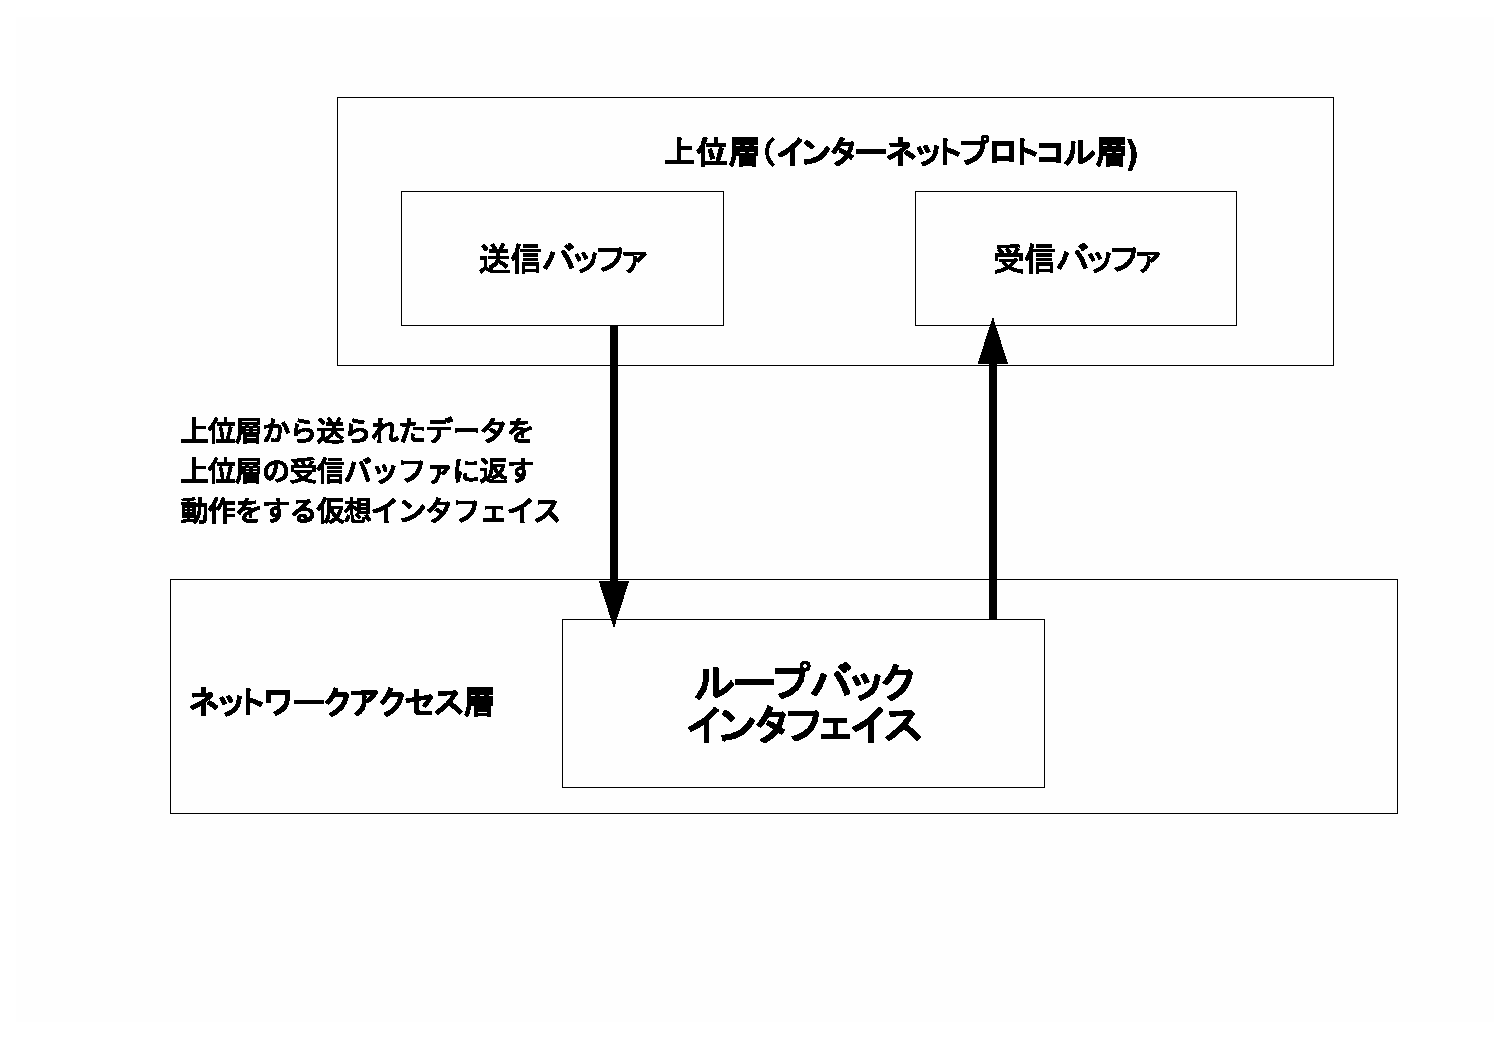
\includegraphics[width=12cm,clip]{draw/loopback.eps}
	\caption{ループバックインタフェイス}
	\label{fig:loopback}
\end{figure}

本章の最後に、他のインタフェイスを区別する必要が無いインタフェイスとして、ループバックインタフェイスについて説明しよう。

あるホストが、自分自身と通信するときに用いられる、ループバックというインタフェイスがある。ループバックインタフェイスは、ネットワークコミュニケーション層に実装される、仮想的なネットワークのインタフェイスである。

ループバックインタフェイスは、上位層から渡されたデータを、同一ホストの上位層の受信バッファに送るサービスをするネットワークコミュニケーション層の実装である。自分の上位層から送信するように渡されたデータを、同じ上位層に返すので、ループバックインタフェイス呼ばれる。
ループバックインタフェイスは、受け取ったデータを外部には送信せず、必ず自分自身の上位層に渡す。
そのため、自分以外のネットワークインタフェイスを区別する必要がない。

また、ループバックインタフェイスは実在するネットワークインタフェイスと対応せず、物理デバイスと対応づけるための名前をもたない。\footnote{ifconfigコマンドでループバックインタフェイスの情報を見ると、MACアドレスは設定されていないことがわかる。}

上位層での宛先が自分自身であるとき、上位層はデータを送信するために、ループバックインタフェイスのサービスを利用する。
そうすることで、上位層のプロトコルで、自分自身と通信をすることが可能となる。この選択は、上位層で、上位層のアドレスと、ネットワークコミュニケーション層のインテフェイスの対応関係の情報によって行われる。

